For experiences, the architecture used is a hierarchical platform. It has 16 nodes interconnected with an Infini Band network. Each node includes  2 Intel(R) Xeon(R) E5220 quad core. Thus, the  total number of cores is 128.

The software used are Linux as operating system, \dague as runtime system and the Intel Mkl library version 11.1 for Blas routines. We used the sequential version of BLAS.

For the experience, we provide a \emph{gemm} peak performance of the patform. It is measured as the best performance obtained by a single core to compute a matrix multiplication using the \emph{gemm} BLAS routine. This measurement is then multiplied by the total number of cores used. It is considered as the practical peak performance of the platform. 

However, the \emph{gemm} peak will never be reached by the LU decomposition algorithm. In order to have a better upper bound for the LU decomposition with partial pivoting, we also implemented an LU decomposition with static pivoting. It is similar to a partial pivoting but without swapping operation. It may be considered a Cholesky's algorithm applied to the two sides of the matrix.


The partial pivoting implemented was run with only 7 cores by node for computation. The eighth core was completely dedicated to the communication. In fact, experiments show that is more efficient to allow one core to manage the huge number of small communications on the panel. Thus, in the figure \ref{fig:pp}, it is showed two \emph{gemm} peaks, one using 8 cores per node and the second using only 7 cores per node.

\dague includes already an implementation of LU decomposition with incremental pivoting. Thus, we use also to compare with the performances obtained of partial pivoting.

To complete the experiences, we also compare results with ScaLAPACK performances. For that, we used the Netlib\footnote{\url{http://www.netlib.org/}} version. ScaLAPACK was run by assigning one process MPI per core.

%\section*{Exploiting hierarchical platform with PTG}



\begin{figure}
\centering
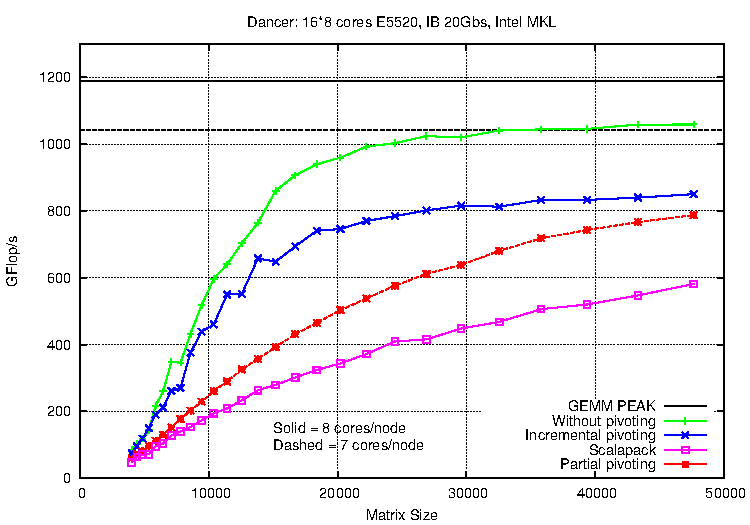
\includegraphics[width=0.8\textwidth]{figures/gepp.pdf}
\caption{Performance of LU decomposition with PTG\label{fig:pp}} 
\end{figure}

 
We implemented Task flow \ref{fig:hybrid_task_flow} for panel factorization and Task flow \ref{fig:update_task_flow} for swapping operations in update. 
We used a 2D block cyclic distribution for matrix. The size of tile used was 200 for \dague and 120 for ScaLAPACK.

For each measurement, we do five iteration of the execution, we do not take in count the maximal and minimal values obtained, We display the average of the three other values. In most of the tests, we obtain a low standard deviation.

The results obtained are encouraging  because our implementation outperform the ScaLAPACK implementation and reached 75\% of the GEMM peak.
However, the incremental pivoting algorithm which enables more parallelism and less synchronization in the panel factorization still provide better performance.
The static pivoting implementation is given here as an upper bound that we hope to reach with our algorithm, but this algorithm cannot be exploited on general cases due to its lack of stability. 

%\section{Exploiting heterogeneous platform with sequential task flow}


%The distributed tests was applied on a machine of 16 nodes of 8 cores each, using an Infini Band network and the Intel MKL library.
%The first experiment applied was to take the static pivoting and plug on it the update engine implemented. Because all communications are done in every case, this test give the cost of the execution of the update engine. The result is showen in the figure \ref{fig:update}. The first remark is that the static pivoting is quickly approaching the gemm peak computer. This can be explained by the fact that all the getrf and trsm operations are recovered by gemm. The second curve is just a little below the first one. Thus, the update engine has a very small impact on the performances despite of its entire execution.  This is a very good result because first the update engine is generic and second its cost is very low.
%\begin{figure}
%\centering
%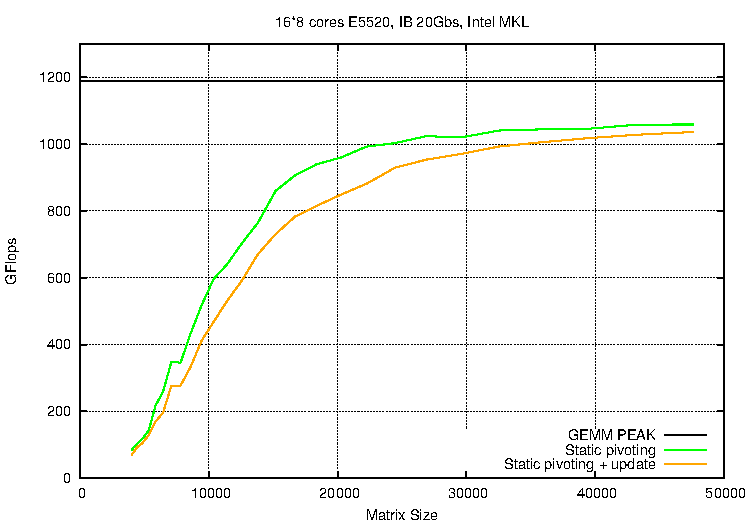
\includegraphics[width=0.8\textwidth]{figures/dgetrf_update_problem.pdf}
%\caption{Impact of the update engine on the performances\label{fig:update}} 
%\end{figure}
%The second experiment applied was the testing of the LU decomposition with partial pivoting implemented. It was compared to the incremental pivoting and the Scalapack implementation. At the moment, the partial pivoting implemented was runned with only 7 cores by node for computation. The eighth core was completly dedicated to the communication. This was necesary to manage the high number of small communications on the panel. In the figure \ref{fig:pp}, it is showed two gemm peak, one using 8 core and the other only 7.
%\begin{figure}
%\centering
%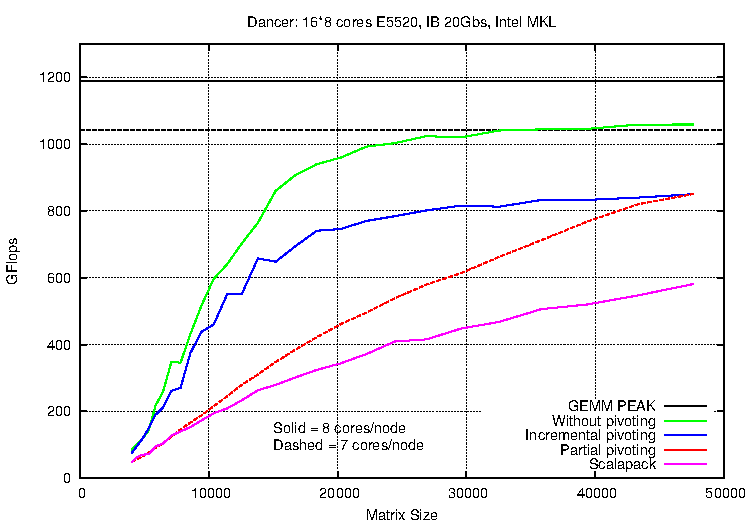
\includegraphics[width=0.8\textwidth]{figures/partial_pivoting_problem.pdf}
%\caption{Impact of the update engine on the performances\label{fig:pp}} 
%\end{figure}
